\documentclass[11pt,border=5pt]{standalone}
\usepackage{amsmath,tikz}
\usepackage[compat=1.1.0]{tikz-feynman}
\usepackage[T1]{fontenc}
\tikzset{
  gluon/.style={draw=black,line width=.65pt,/tikzfeynman/gluon},
  cut/.style={draw=black,line width=.5pt,dash pattern=on 1.3pt off 1.7pt}}
\begin{document}
% Representative real cut entering I_gg. Operator endpoints, gauge links,
% other diagrams and subtraction terms are suppressed in this illustration.
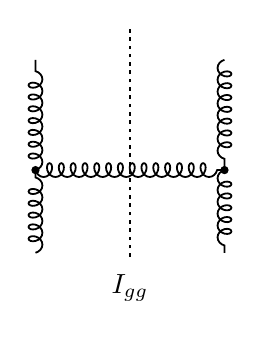
\begin{tikzpicture}
  \draw[cut] (1.2,-.05)--(1.2,2.85);
  \draw[gluon] (0,0)--(0,1.05);
  \draw[gluon] (0,1.05)--(0,2.45);
  \draw[gluon] (2.4,2.45)--(2.4,1.05);
  \draw[gluon] (2.4,1.05)--(2.4,0);
  \draw[gluon] (0,1.05)--(2.4,1.05);
  \fill (0,1.05) circle (1.5pt);
  \fill (2.4,1.05) circle (1.5pt);
  \node at (1.2,-.45) {$I_{gg}$};
\end{tikzpicture}
\end{document}
